\documentclass[12pt,a4paper]{article}

\usepackage[utf8]{inputenc}
\usepackage[T2A]{fontenc}
\usepackage[russian]{babel}
\usepackage{amsmath,amssymb}
\usepackage{graphicx}
\usepackage{booktabs}
\usepackage{geometry}
\geometry{top=2cm,bottom=2cm,left=2.5cm,right=1.5cm}
\usepackage{float}
\usepackage{indentfirst}

\title{\textbf{Лабораторная работа 1.2.3}\\
Определение моментов инерции твёрдых тел с помощью трифилярного подвеса}

\author{
    Студент \underline{Шеховцов Василий Максимович}\\
    Группа \underline{Б03-601}\\
    Преподаватель \underline{Ивлев Д.А.}
}

\date{Московский Физико-технический институт\\
(национальный исследовательский университет)\\
14 октября 2026 г.}

\begin{document}
\maketitle

\section*{Цель работы}

Измерение момента инерции ряда тел и сравнение результатов с теоретическими формулами; проверка аддитивности моментов инерции и справедливости формулы Гюйгенса--Штейнера.

\section*{Оборудование}

\begin{itemize}
    \item трифилярный подвес;
    \item штангенциркуль;
    \item секундомер;
    \item счётчик числа колебаний (осветитель, фотоэлемент, пересчётное устройство);
    \item набор тел (крышка, полый цилиндр, разрезанный диск).
\end{itemize}

\section*{Теоретическая часть}

Инерционность при вращении тела относительно оси определяется моментом инерции тела относительно этой оси. Момент инерции твёрдого тела относительно неподвижной оси вращения вычисляется по формуле
\begin{equation}
    I = \int \rho^2 \, dm,
\end{equation}
где \(\rho\) --- расстояние элемента массы \(dm\) от оси вращения; интегрирование проводится по всей массе тела.

Для однородных тел простой формы момент инерции можно вычислить, для неоднородных тел и тел сложной формы его определяют экспериментально с помощью трифилярного подвеса (рис.~\ref{fig:trifilar}). Он состоит из неподвижной верхней платформы \(P\) и подвешенной к ней на трёх симметрично расположенных нитях \(AA'\), \(BB'\), \(CC'\) вращающейся нижней платформы \(P'\). Колебания возбуждаются небольшим поворотом верхней платформы; нижняя при этом остаётся неподвижной по вертикали, и возникают крутильные колебания, число которых считает фотоэлемент со счётчиком. Радиус окружности крепления нитей на верхней платформе \(r\), на нижней \(R\), расстояние между платформами в положении равновесия \(z_0\).

\begin{figure}[H]
    \centering
    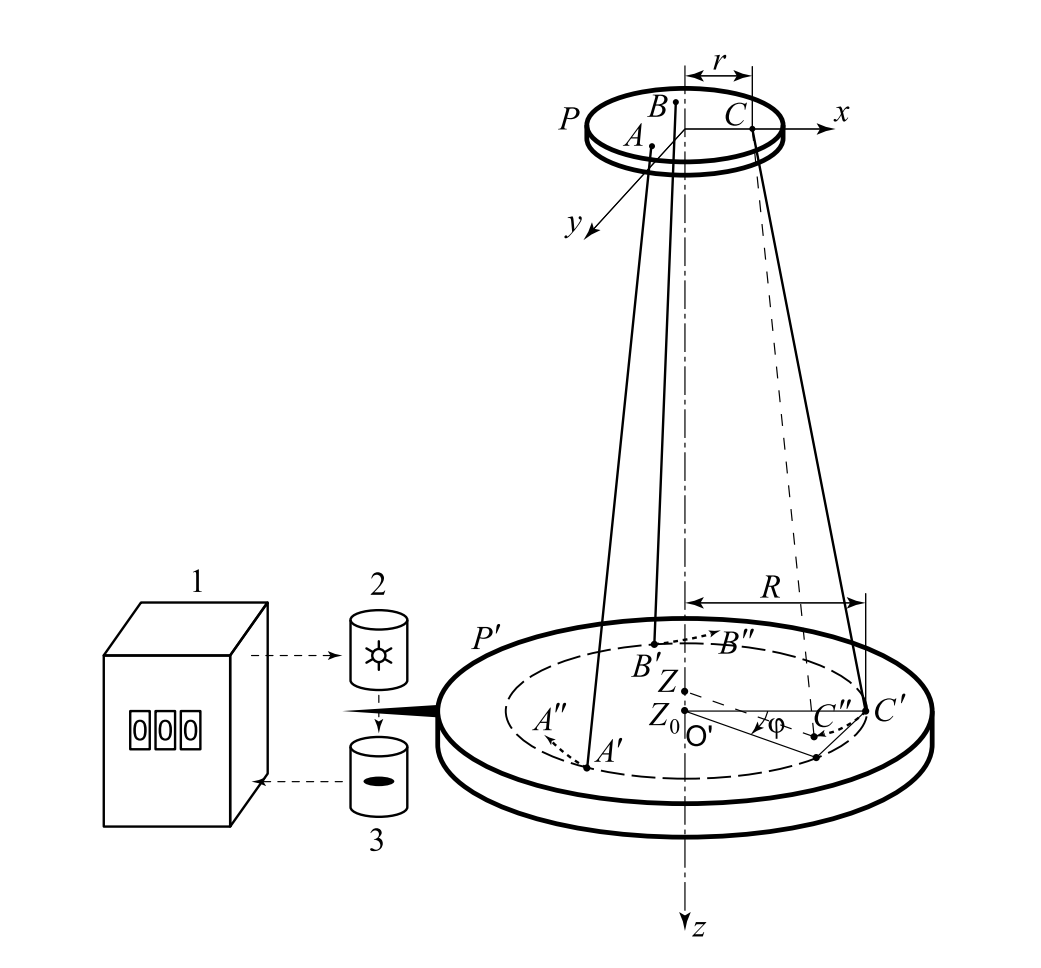
\includegraphics[width=0.62\textwidth]{trifilar.png}
    \caption{Трифилярный подвес: \(P\), \(P'\)~--- верхняя и нижняя платформы, 1~--- пересчётное устройство, 2~--- осветитель, 3~--- фотоэлемент}
    \label{fig:trifilar}
\end{figure}

Если пренебречь потерями энергии на трение, уравнение сохранения энергии при колебаниях имеет вид
\begin{equation}
    \frac{I\dot{\varphi}^2}{2} + mg(z_0 - z) = E,
\end{equation}
где \(I\) --- момент инерции платформы с телом, \(m\) --- их общая масса, \(\varphi\) --- угол поворота от положения равновесия, \(z_0\) --- координата центра нижней платформы при равновесии, \(z\) --- та же координата при повороте на угол \(\varphi\).

В системе координат, связанной с верхней платформой, верхний конец нити \(C\) имеет координаты \((r,0,0)\), нижний \(C'\) при равновесии \((R,0,z_0)\), а при повороте на угол \(\varphi\) --- \(C''(R\cos\varphi,\,R\sin\varphi,\,z)\). Расстояние между \(C\) и \(C''\) равно длине нити \(L\):
\begin{equation}
    (R\cos\varphi - r)^2 + R^2\sin^2\varphi + z^2 = L^2.
\end{equation}
При малых углах \(\cos\varphi \approx 1 - \varphi^2/2\), поэтому
\begin{equation}
    z^2 = z_0^2 - 2Rr(1-\cos\varphi) \approx z_0^2 - Rr\varphi^2, \qquad z \approx z_0 - \frac{Rr\varphi^2}{2z_0}.
\end{equation}

Подставляя \(z\) в уравнение энергии и дифференцируя по времени, получаем уравнение гармонических колебаний
\begin{equation}
    I\ddot{\varphi} + mg\frac{Rr}{z_0}\varphi = 0,
\end{equation}
откуда период равен
\begin{equation}
    T = 2\pi\sqrt{\frac{Iz_0}{mgRr}}.
\end{equation}
Из этой формулы находим момент инерции:
\begin{equation}
    I = \frac{mgRrT^2}{4\pi^2 z_0} = k m T^2,
\end{equation}
где \(k = \dfrac{gRr}{4\pi^2 z_0}\) --- постоянная установки.

Момент инерции тела находится по аддитивности: из момента инерции платформы с телом вычитается момент инерции пустой платформы. Формулы выведены в предположении малого затухания: время \(\tau\) уменьшения амплитуды в 2--3 раза должно быть много больше периода, \(\tau \gg T\). Период рекомендуется определять с относительной погрешностью 0,5\%; число колебаний выбирается исходя из этой погрешности и погрешности измерения времени.

\section*{Экспериментальная часть}

\section{Константа установки и её погрешность}

Параметры установки: \(R = 114.6\) мм, \(r = 30.2\) мм, \(z_0 = 220\) см \(= 2.20\) м (погрешность \(\sigma_{z_0} = 0.5\) см).

\begin{equation}
    k = \frac{g R r}{4\pi^2 z_0} = \frac{9.81 \cdot 0.1146 \cdot 0.0302}{4 \pi^2 \cdot 2.20} \approx 3.909 \cdot 10^{-4} \text{ м}^2/\text{с}^2
\end{equation}

Относительная погрешность \(k\):
\begin{equation}
\begin{split}
    \frac{\sigma_k}{k} &= \sqrt{\left(\frac{\sigma_{R}}{R}\right)^2 + \left(\frac{\sigma_{r}}{r}\right)^2 + \left(\frac{\sigma_{z_0}}{z_0}\right)^2} = \\
    &= \sqrt{\left(\frac{0.0005}{0.1146}\right)^2 + \left(\frac{0.0003}{0.0302}\right)^2 + \left(\frac{0.005}{2.20}\right)^2} \approx 0.0111 \ (1.11\%)
\end{split}
\end{equation}

Абсолютная погрешность: \(\sigma_k = 3.909 \cdot 10^{-4} \cdot 0.0111 \approx 0.043 \cdot 10^{-4}\).
\begin{center}
\(k = (3.909 \pm 0.043) \cdot 10^{-4} \text{ м}^2/\text{с}^2\)
\end{center}

\section{Пустая платформа (расчёт \(I_0\))}

Данные для амплитуды 15\(^\circ\).
\begin{table}[H]
    \centering
    \caption{Измерения периода пустой платформы (амплитуда 15\(^\circ\))}
    \begin{tabular}{cccc}
        \toprule
        № & Время \(t_i\), с & Число колебаний \(N_i\) & Период \(T_i\), с \\
        \midrule
        1 & 65.26 & 15 & 4.3507 \\
        2 & 65.05 & 15 & 4.3367 \\
        3 & 70.50 & 16 & 4.4063 \\
        4 & 86.79 & 20 & 4.3395 \\
        5 & 43.82 & 10 & 4.3820 \\
        \bottomrule
    \end{tabular}
\end{table}

Средний период: \(\bar{T}_0 = 4.363\) с.
Случайная погрешность (среднеквадратичное отклонение среднего по 5 измерениям): \(\sigma_{T_0}^{\text{случ}} \approx 0.013\) с.
Систематическая (секундомер \(0.01\) с, \(N=15\)): \(\sigma_{T_0}^{\text{сист}} \approx 0.0007\) с.
Полная погрешность: \(\sigma_{T_0} = \sqrt{0.013^2 + 0.0007^2} \approx 0.013\) с (относительная \(\approx 0.3\%\), меньше рекомендуемых 0.5\%).

Момент инерции платформы (масса \(m_0 = 1.0668\) кг):
\begin{equation}
    I_0 = k m_0 \bar{T}_0^2 = 3.909 \cdot 10^{-4} \cdot 1.0668 \cdot 4.363^2 \approx 7.94 \cdot 10^{-3} \text{ кг}\cdot\text{м}^2
\end{equation}

Погрешность \(I_0\):
\begin{equation}
\begin{split}
    \frac{\sigma_{I_0}}{I_0} &= \sqrt{\left(\frac{\sigma_k}{k}\right)^2 + \left(\frac{\sigma_{m_0}}{m_0}\right)^2 + \left(2\frac{\sigma_{T_0}}{\bar{T}_0}\right)^2} = \\
    &= \sqrt{0.0111^2 + \left(\frac{0.0005}{1.0668}\right)^2 + (2 \cdot 0.0031)^2} \approx 0.0127 \ (1.27\%)
\end{split}
\end{equation}
\begin{center}
\(I_0 = (7.94 \pm 0.10) \cdot 10^{-3} \text{ кг}\cdot\text{м}^2\)
\end{center}

\section{Полый цилиндр (ободок)}
Масса \(m_1 = 0.7476\) кг. Средний период \(\bar{T}_1 = 4.195\) с, \(\sigma_{T_1} = 0.035\) с (отн. 0.83\%, больше рекомендуемых 0.5\%).
Момент инерции системы \((m_0 + m_1 = 1.8144\) кг\()\):
\begin{equation}
    I_{\text{сист}} = 3.909 \cdot 10^{-4} \cdot 1.8144 \cdot 4.195^2 \approx 12.48 \cdot 10^{-3} \text{ кг}\cdot\text{м}^2
\end{equation}
Погрешность \(I_{\text{сист}}\): \(\sigma \approx 0.25 \cdot 10^{-3}\) кг·м\(^2\).
Момент инерции самого ободка:
\begin{equation}
    I_{\text{ободок}} = 12.48 \cdot 10^{-3} - 7.94 \cdot 10^{-3} = 4.54 \cdot 10^{-3} \text{ кг}\cdot\text{м}^2
\end{equation}
Погрешность: \(\sigma_{I_1} = \sqrt{0.25^2 + 0.10^2} \cdot 10^{-3} \approx 0.27 \cdot 10^{-3}\).
\begin{center}
\(I_{\text{ободок}} = (4.54 \pm 0.27) \cdot 10^{-3} \text{ кг}\cdot\text{м}^2\)
\end{center}

\section{Крышка}
Масса \(m_2 = 0.59\) кг. Средний период \(\bar{T}_2 = 3.936\) с, \(\sigma_{T_2} = 0.002\) с (отн. 0.05\%).
Момент инерции системы \((m_0 + m_2 = 1.6568\) кг\()\):
\begin{equation}
    I_{\text{сист}} = 3.909 \cdot 10^{-4} \cdot 1.6568 \cdot 3.936^2 \approx 10.03 \cdot 10^{-3} \text{ кг}\cdot\text{м}^2
\end{equation}
Погрешность \(I_{\text{сист}}\): \(\sigma \approx 0.11 \cdot 10^{-3}\) кг·м\(^2\).
Момент инерции крышки:
\begin{equation}
    I_{\text{крышка}} = 10.03 \cdot 10^{-3} - 7.94 \cdot 10^{-3} = 2.10 \cdot 10^{-3} \text{ кг}\cdot\text{м}^2
\end{equation}
Погрешность: \(\sigma_{I_2} = \sqrt{0.11^2 + 0.10^2} \cdot 10^{-3} \approx 0.15 \cdot 10^{-3}\).
\begin{center}
\(I_{\text{крышка}} = (2.10 \pm 0.15) \cdot 10^{-3} \text{ кг}\cdot\text{м}^2\)
\end{center}

\section{Проверка аддитивности}
Масса обоих тел вместе с платформой \(m_0 + m_1 + m_2 = 2.4044\) кг, средний период \(\bar{T}_{12} = 3.914\) с.
\begin{equation}
    I_{12}^{\text{эксп}} = 3.909 \cdot 10^{-4} \cdot 2.4044 \cdot 3.914^2 - I_0 = 14.40 \cdot 10^{-3} - 7.94 \cdot 10^{-3} = 6.46 \cdot 10^{-3} \text{ кг}\cdot\text{м}^2
\end{equation}
Сумма моментов инерции:
\begin{equation}
    I_{12}^{\text{теор}} = I_{\text{ободок}} + I_{\text{крышка}} = (4.54 + 2.10) \cdot 10^{-3} = 6.64 \cdot 10^{-3} \text{ кг}\cdot\text{м}^2
\end{equation}
Разница: \(\Delta = |6.46 - 6.64| \cdot 10^{-3} = 0.18 \cdot 10^{-3}\) кг·м\(^2\). Погрешность суммы: \(\sigma = \sqrt{0.27^2 + 0.15^2} \cdot 10^{-3} \approx 0.31 \cdot 10^{-3}\).

\textbf{Вывод:} разница (\(0.18 \cdot 10^{-3}\)) меньше погрешности суммы (\(0.31 \cdot 10^{-3}\)), аддитивность выполняется.

\section{Расчётные моменты инерции и сравнение с измеренными}
Для расчёта ободок принят тонким кольцом радиуса \(R_1 = 7.5\) см, крышка~--- однородным диском диаметром \(17.8\) см (\(R_2 = 8.9\) см). Погрешности: радиусов \(0.05\) см, масс \(0.0005\) кг.
\begin{equation}
    I_1^{\text{расч}} = m_1 R_1^2 = 0.7476 \cdot 0.075^2 \approx 4.21 \cdot 10^{-3} \text{ кг}\cdot\text{м}^2,
\end{equation}
\begin{equation}
    I_2^{\text{расч}} = \frac{m_2 R_2^2}{2} = \frac{0.590 \cdot 0.089^2}{2} \approx 2.34 \cdot 10^{-3} \text{ кг}\cdot\text{м}^2.
\end{equation}
Погрешности \(\sigma_I = I\sqrt{(\sigma_m/m)^2 + (2\sigma_R/R)^2}\): \(\sigma_{I_1} \approx 0.06 \cdot 10^{-3}\), \(\sigma_{I_2} \approx 0.03 \cdot 10^{-3}\) кг·м\(^2\).

\begin{table}[H]
    \centering
    \caption{Измеренные и расчётные моменты инерции, \(10^{-3}\) кг·м\(^2\)}
    \begin{tabular}{lccc}
        \toprule
        Тело & \(I_{\text{изм}}\) & \(I_{\text{расч}}\) \\
        \midrule
        Ободок & \(4.54 \pm 0.27\) & \(4.21 \pm 0.06\)  \\
        Крышка & \(2.10 \pm 0.15\) & \(2.34 \pm 0.03\) \\
        Ободок + крышка & \(6.46 \pm 0.31\) & \(6.54 \pm 0.06\) \\
        
        \bottomrule
    \end{tabular}
\end{table}

\section{Разрезанный диск}
Масса двух половинок \(m_{\text{д}} = 1.4418\) кг, масса системы \(m_0 + m_{\text{д}} = 2.5086\) кг. На платформе нанесены риски (концентрические окружности) с шагом \(0.005\) м. Радиус диска равен 9 рискам: \(R = 9 \cdot 0.005 = 0.045\) м, то есть при сомкнутых половинках внешний край лежит на 9-й риске. Половинки раздвигаются симметрично до \(N\)-й риски, поэтому смещение каждой из них от сомкнутого положения \(h = (N-9)\cdot 0.005\) м. Период \(T = t/20\) (20 колебаний). Момент инерции диска при каждом \(h\):
\begin{equation}
    I_{\text{диска}} = k (m_0 + m_{\text{д}}) \left(\frac{t}{20}\right)^2 - I_0
\end{equation}

\begin{table}[H]
    \centering
    \caption{Зависимость момента инерции разрезанного диска от смещения \(h\)}
    \begin{tabular}{cccccc}
        \toprule
        \(N\) рисок & \(h\), м & \(h^2\), м\(^2\) & Время \(t\), с & Период \(T\), с & \(I_{\text{диска}}\), \(10^{-3}\) кг·м\(^2\) \\
        \midrule
        9 & 0.000 & 0.000000 & 62.39 & 3.1195 & 1.60 \\
        10 & 0.005 & 0.000025 & 62.60 & 3.1300 & 1.67 \\
        11 & 0.010 & 0.000100 & 62.81 & 3.1405 & 1.73 \\
        12 & 0.015 & 0.000225 & 63.21 & 3.1605 & 1.86 \\
        13 & 0.020 & 0.000400 & 64.14 & 3.2070 & 2.15 \\
        14 & 0.025 & 0.000625 & 65.20 & 3.2600 & 2.48 \\
        15 & 0.030 & 0.000900 & 66.49 & 3.3245 & 2.90 \\
        16 & 0.035 & 0.001225 & 67.56 & 3.3780 & 3.25 \\
        17 & 0.040 & 0.001600 & 68.96 & 3.4480 & 3.72 \\
        18 & 0.045 & 0.002025 & 71.34 & 3.5670 & 4.54 \\
        \bottomrule
    \end{tabular}
\end{table}

График зависимости \(I_{\text{диска}}\) от \(h^2\) построен в Python (рис.~\ref{fig:disk}); сплошная прямая найдена методом наименьших квадратов, пунктир~--- теоретическая зависимость.

\begin{figure}[H]
    \centering
    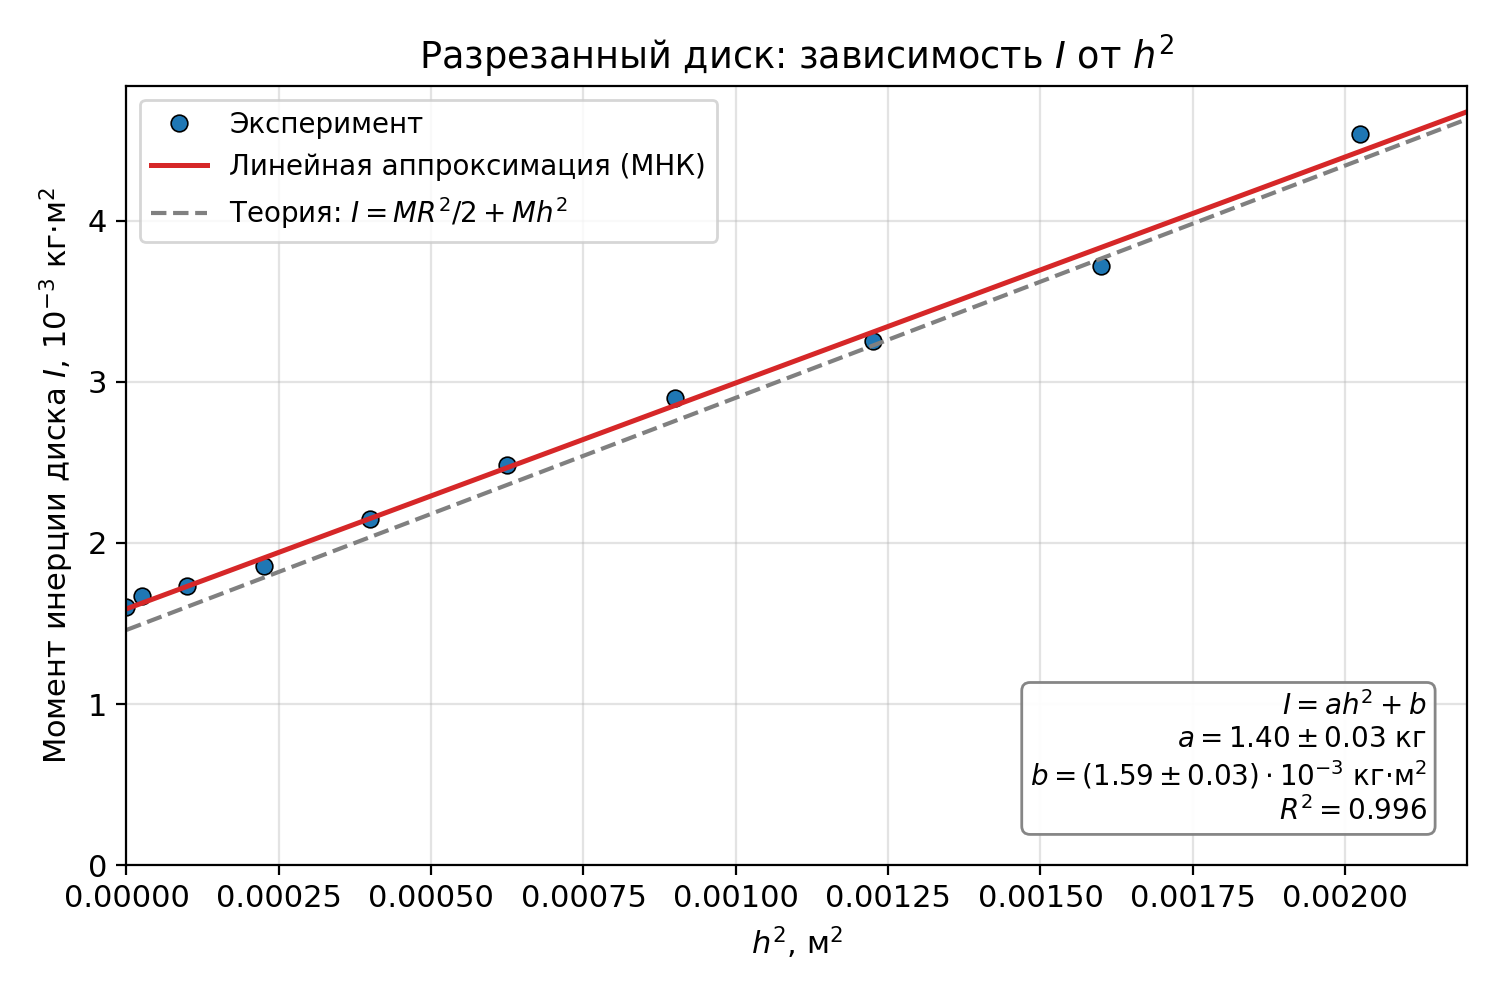
\includegraphics[width=0.85\textwidth]{graph_disk.png}
    \caption{Зависимость момента инерции разрезанного диска от квадрата смещения \(h\)}
    \label{fig:disk}
\end{figure}

Параметры аппроксимации \(I = a h^2 + b\): \(a = 1.403 \pm 0.031\) кг, \(b = (1.59 \pm 0.03) \cdot 10^{-3}\) кг·м\(^2\), коэффициент детерминации \(R^2 = 0.996\).

По формуле Гюйгенса--Штейнера \(I = I_{\text{д0}} + m_{\text{д}} h^2\), где \(I_{\text{д0}} = m_{\text{д}}R^2/2\). Наклон прямой должен быть равен массе диска: получено \(a = 1.403 \pm 0.031\) кг, масса \(m_{\text{д}} = 1.442\) кг; разница \(0.039\) кг составляет \(1.2\sigma\), то есть наклон совпадает с массой в пределах погрешности. Теоретический момент диска \(I_{\text{д0}} = 1.4418 \cdot 0.045^2/2 = 1.46 \cdot 10^{-3}\) кг·м\(^2\); из аппроксимации \(b = 1.59 \cdot 10^{-3}\) кг·м\(^2\), отличие \(0.13 \cdot 10^{-3}\) кг·м\(^2\) сопоставимо с погрешностью \(I_0\) (\(0.10 \cdot 10^{-3}\) кг·м\(^2\)), так как \(b\) получен вычитанием \(I_0\).

\section*{Вывод}
В ходе работы были измерены моменты инерции платформы \((7.94 \pm 0.10) \cdot 10^{-3}\) кг·м\(^2\), ободка \((4.54 \pm 0.27) \cdot 10^{-3}\) кг·м\(^2\) и крышки \((2.10 \pm 0.15) \cdot 10^{-3}\) кг·м\(^2\). Момент инерции системы из двух тел отличается от суммы моментов отдельных тел на \(0.18 \cdot 10^{-3}\) кг·м\(^2\), что меньше погрешности \(0.31 \cdot 10^{-3}\) кг·м\(^2\): аддитивность выполняется. Для разрезанного диска момент инерции растёт с \(h^2\) линейно (\(R^2 = 0.996\)): наклон \(a = 1.403 \pm 0.031\) кг совпадает с массой диска \(1.442\) кг в пределах погрешности, то есть формула Гюйгенса--Штейнера \(I = I_{\text{д0}} + m_{\text{д}} h^2\) подтверждается.

\end{document}